\chapter{Конструкторская часть}
В данном разделе будут реализованы схемы алгоритмов умножения матриц, приведено описание используемых типов данных, а также описана структура программного обеспечения.

\section{Требования к программному обеспечению}\label{section:requirements_1}
К программе предъявлен ряд функциональных требований:
\begin{itemize}
    \item на вход подаются две матрицы;
    \item матрицы располагаются в файлах, с расширением \texttt{*.txt}.
    \item на выходе~--- матрица, являющаяся результатом умножения матриц.
\end{itemize}

К программе предъявлен ряд требований:
\begin{itemize}
	\item наличие интерфейса для выбора действия;
	\item наличие функциональных замеров процессорного времени выполнения алгоритмов умножения матриц;
	\item замеры процессорного времени выполнятся только для квадратных матриц.
\end{itemize}

\section{Разработка алгоритмов}
TODO

На вход алгоритмов подаются строки $S_1$ и $S_2$.

На рисунке \ref{fig:Liter} представлена схема алгоритма поиска расстояния Левенштейна.

На рисунках \ref{fig:DLiter}--\ref{fig:DLrechash} представлены схемы алгоритмов поиска Дамерау~---~Левенштейна.

\begin{figure}[h]
	\centering
	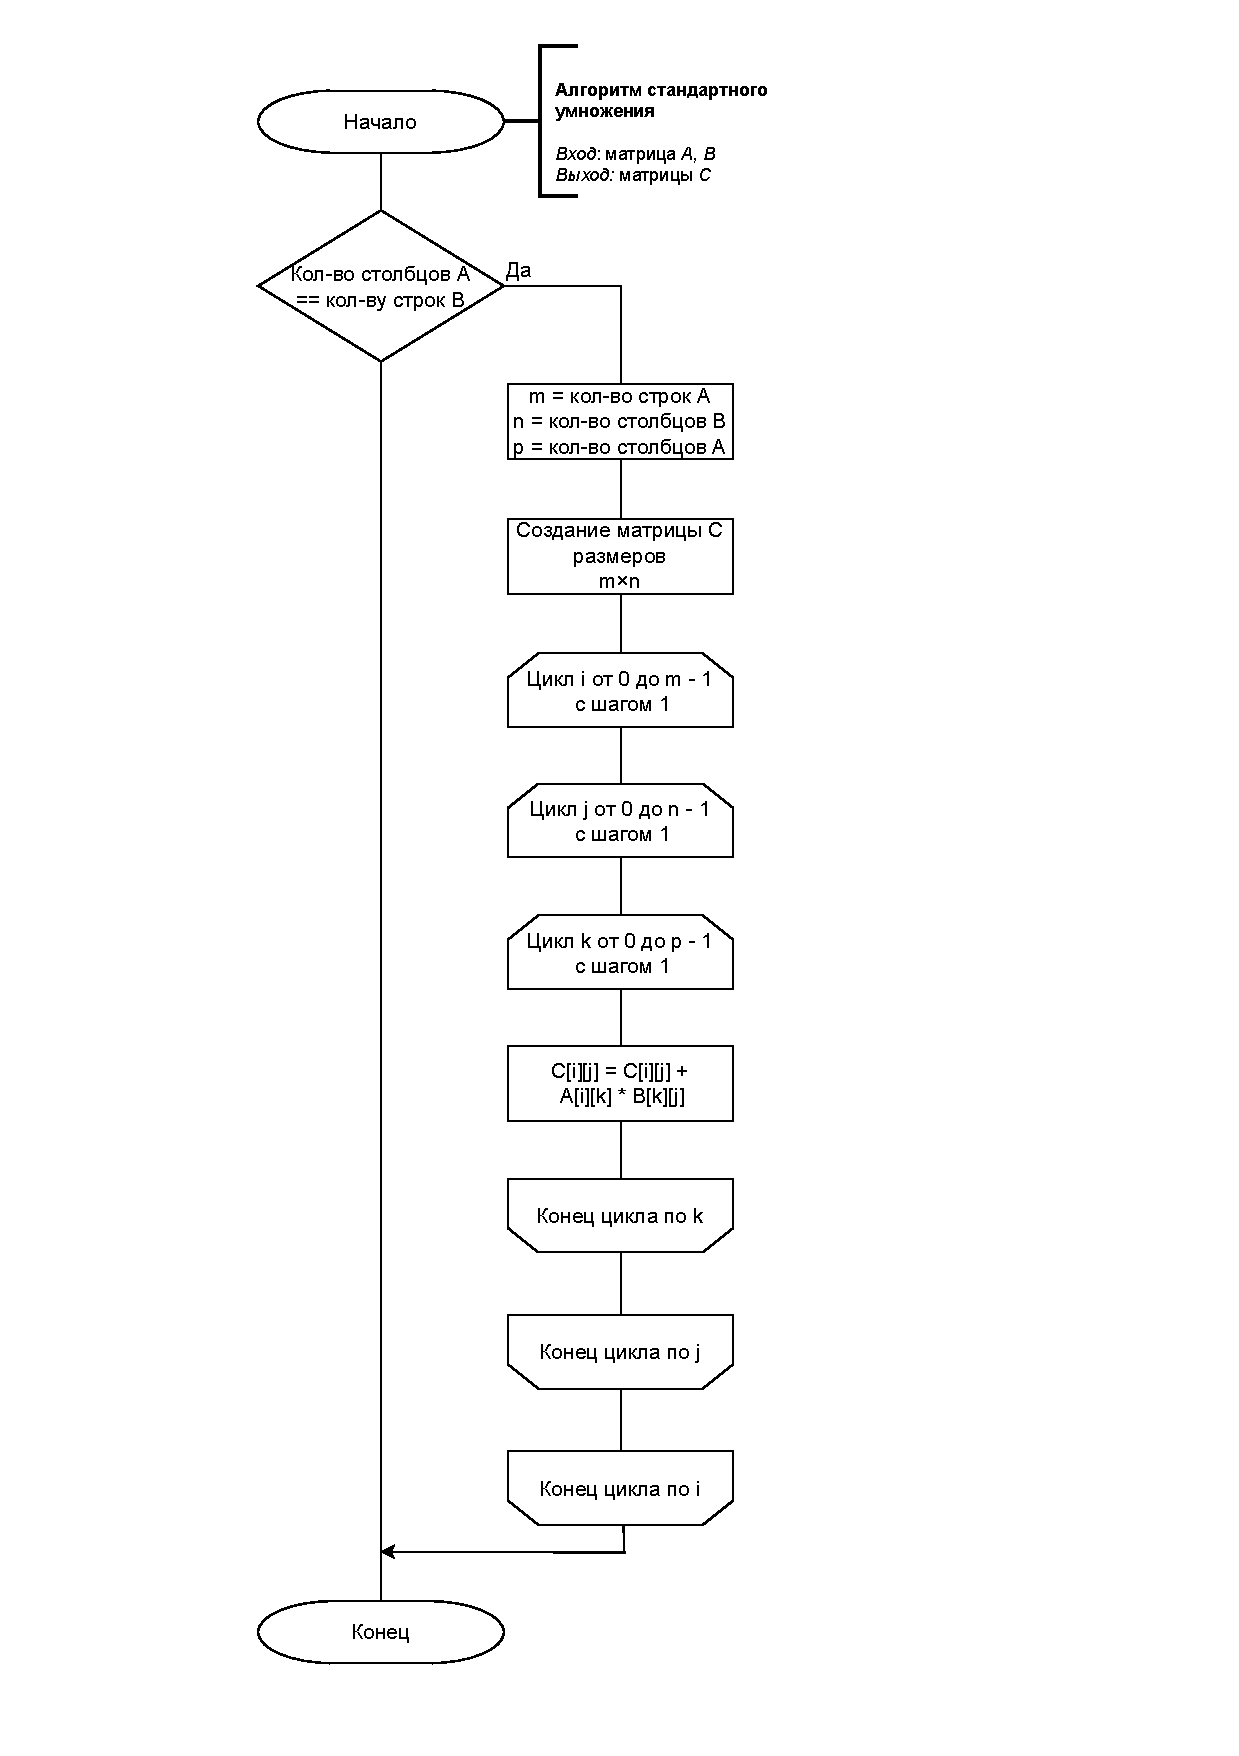
\includegraphics[height=0.7\textheight, page=1]{img/algorithms.pdf}
	\caption{Схема нерекурсивного алгоритма нахождения расстояния Левенштейна}
	\label{fig:Liter}
\end{figure}

\clearpage

\begin{figure}[h]
	\centering
	\includegraphics[height=0.9\textheight, page=2]{img/algorithms.pdf}
	\caption{Схема нерекурсивного алгоритма нахождения расстояния Дамерау~---~Левенштейна}
	\label{fig:DLiter}
\end{figure}

\clearpage

\begin{figure}[h]
	\centering
	\includegraphics[height=0.9\textheight, page=3]{img/algorithms.pdf}
	\caption{Схема рекурсивного алгоритма нахождения расстояния Дамерау~---~Левенштейна}
	\label{fig:DLrec}
\end{figure}

\clearpage

\begin{figure}[h]
	\centering
	\includegraphics[height=0.9\textheight, page=4]{img/algorithms.pdf}
	\caption{Схема алгоритма вызова рекурсивного алгоритма нахождения расстояния Дамерау~---~Левенштейна с кешированием}
	\label{fig:DLrechashDecor}
\end{figure}

\begin{figure}[h]
	\centering
	\includegraphics[height=0.9\textheight, page=5]{img/algorithms.pdf}
	\caption{Схема рекурсивного алгоритма нахождения расстояния Дамерау~---~Левенштейна с кешированием}
	\label{fig:DLrechash}
\end{figure}

\clearpage

\section{Описание используемых типов данных}

При реализации алгоритмов будут использованы следующие структуры данных:

\begin{itemize}
	\item \textit{строка}~--- массив символов типа $wchar{\_}t$;
	\item \textit{длина строки}~--- целое число типа $int$;
	\item \textit{матрица}~--- двумерный массив значений типа $int$.
\end{itemize}

\section{Модель вычислений для проведения оценки трудоемкости алгоритмов}

\section{Трудоемкость алгоритмов}

\subsection*{Классический алгоритм}
\subsection*{Алгоритм Винограда}
\subsection*{Оптимизированный алгоритм Винограда}
	
\section*{Вывод}

В данном разделе на основе теоретических данных были перечислены требования к ПО, а также были построены схемы требуемых алгоритмов на основе теоретических данных, полученных на этапе анализа.